\chapter{Diffie-Hellman Schlüsselaustausch}
\section{Ablauf}
Der Diffie-Hellman Schlüsselaustausch (asymmetrisch) verwendet das \textbf{modulare Potenzieren}.

\begin{figure}[H]
	\centering
	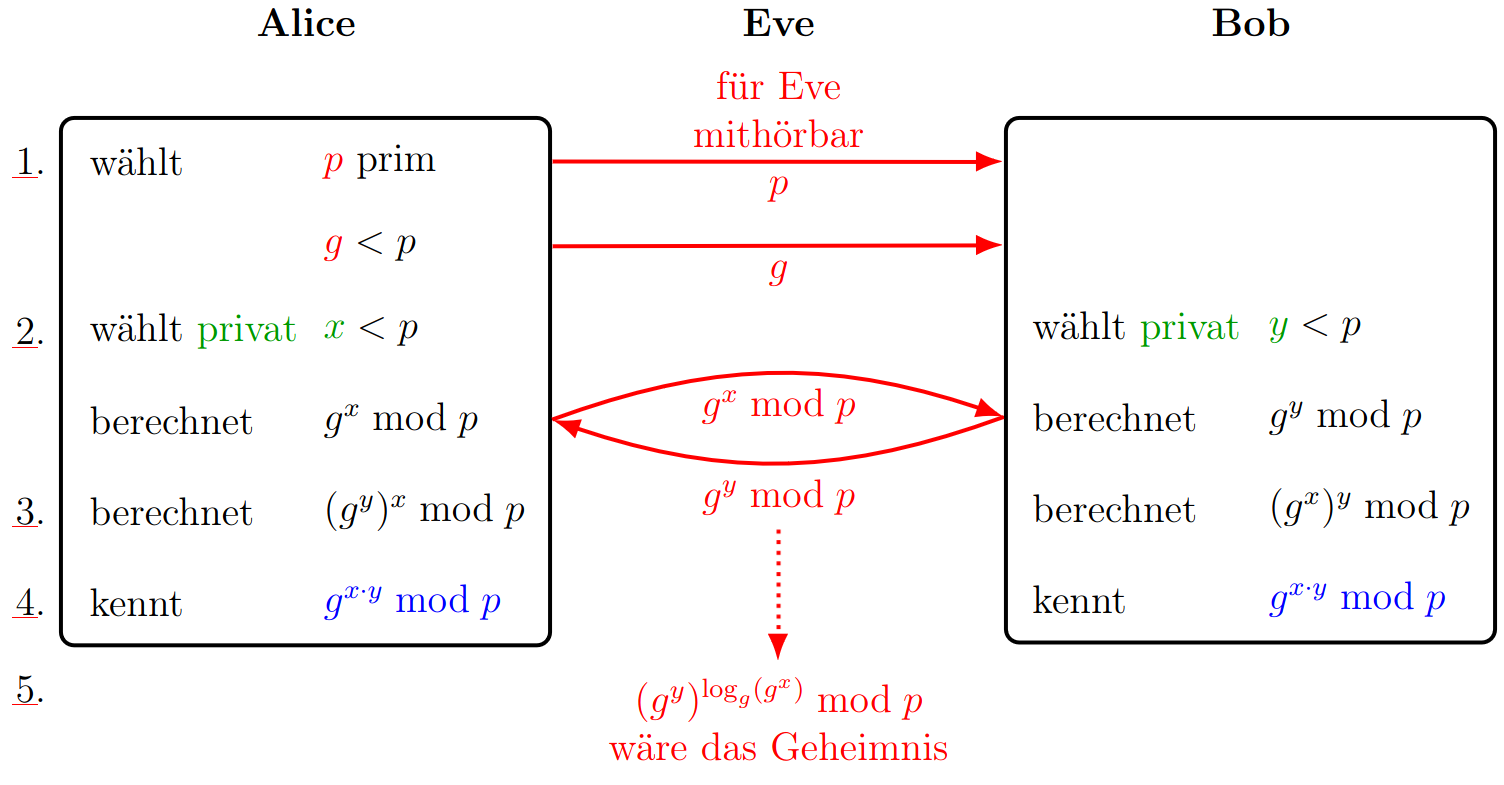
\includegraphics[width=1.0\linewidth]{figures/diffhell.png}
	\caption{Diffie-Hellman Schlüsselaustausch}
\end{figure}
\begin{enumerate}
	\item Es wird eine Primzahl $p$ und (idealerweise) ein Generator $g < p$ ausgewählt und veröffentlicht.
	\item Beide Parteien wählen eine private Zahl $x$ bzw. $y$ welche $< p$ sind aus und Potenzieren den Generator $g$ hoch $x/y$
	\item Das Ergebnis wird ausgetauscht und wieder mit ihrer privaten Zahl ($x/y$) potenziert.
	\item da $(g^x)^y = g^{x \cdot y} = (g^y)^x$ wurde der Schlüssel bei beiden Parteien generiert, ohne dass jemand anders es mitbekommen hat
	\item Wenn \textit{Eve} effizient den diskreten Logarithmus berechnen könnte, könnte sie die Verschlüsselung mit den gegebenen veröffentlichten Informationen knacken. \textbf{Da der diskrete Logarithmus enorm aufwendig ist, kann Eve die Verschlüsselung nicht knacken}
\end{enumerate}

\section{Allgemein}
Diffie-Hellman tauscht also die Schlüssel aus, indem man sie mit gegebenen Informationen berechnet/generiert. \\
Diffie-Hellman gilt als sicher, wenn $g$, $x$, und $y$ mindestens 1024 Bit-Zahlen sind. \\
\textbf{Die Sicherheit von asymmetrischen Verfahren, basiert darauf, dass es (derzeit) keine effizienten Verfahren zur Umkehrung oder keine Quantencomputer gibt}

\section{Man-in-the-Middle}
Diffie-Hellman bietet keinen Schutz von Man-in-the-Middle Angriffe.
\begin{figure}[H]
	\centering
	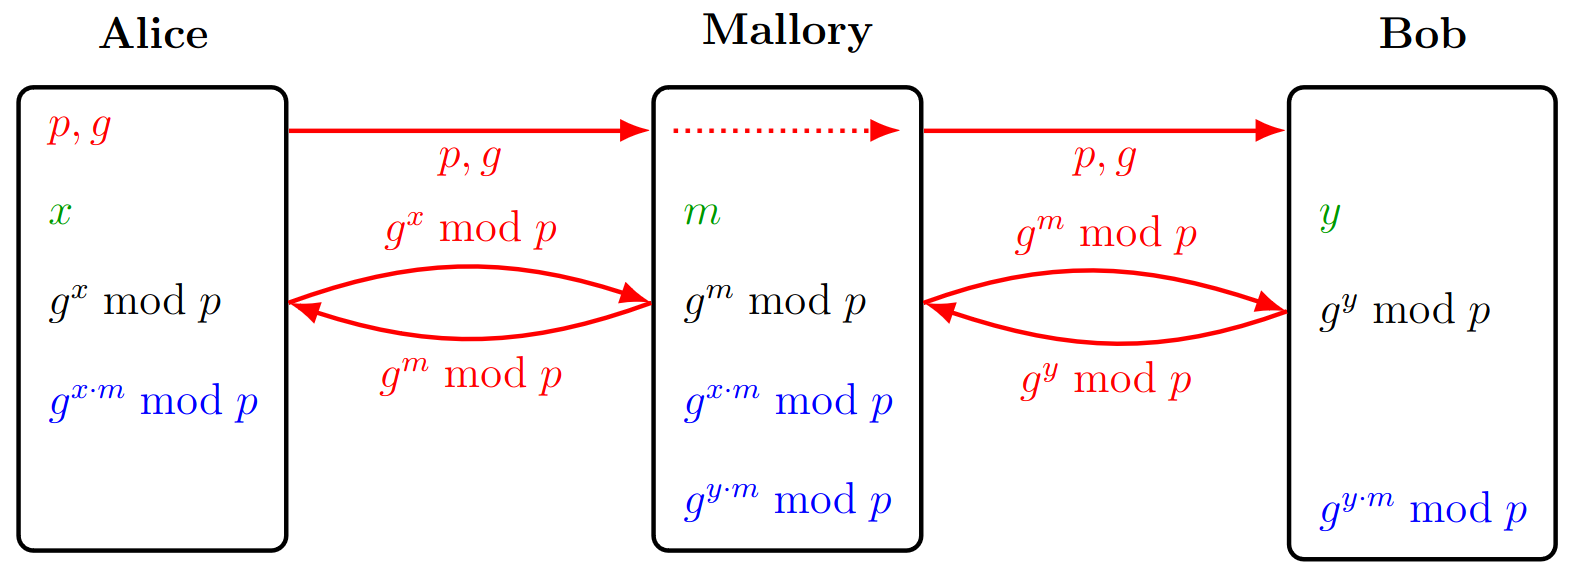
\includegraphics[width=1.0\linewidth]{figures/diffhell_mitm.png}
	\caption{Diffie-Hellman Man-in-the-Middle}
\end{figure}